% Created 2021-01-24 Sun 22:50
% Intended LaTeX compiler: pdflatex
\documentclass[11pt]{article}
\usepackage[utf8]{inputenc}
\usepackage[T1]{fontenc}
\usepackage{graphicx}
\usepackage{grffile}
\usepackage{longtable}
\usepackage{wrapfig}
\usepackage{rotating}
\usepackage[normalem]{ulem}
\usepackage{amsmath}
\usepackage{textcomp}
\usepackage{amssymb}
\usepackage{capt-of}
\usepackage{hyperref}
\usepackage{minted}
\hypersetup{colorlinks=true, linkcolor=black, filecolor=red, urlcolor=blue}
\usepackage[turkish]{babel}
\author{Eren Hatırnaz}
\date{4 Ağustos 2019}
\title{Yazılım Gündemi - 4\\\medskip
\large 29 Temmuz - 4 Ağustos 2019}
\hypersetup{
 pdfauthor={Eren Hatırnaz},
 pdftitle={Yazılım Gündemi - 4},
 pdfkeywords={},
 pdfsubject={},
 pdfcreator={Emacs 27.1 (Org mode 9.3)},
 pdflang={Turkish}}
\begin{document}

\maketitle
\tableofcontents \clearpage\shorthandoff{=}

\begin{center}
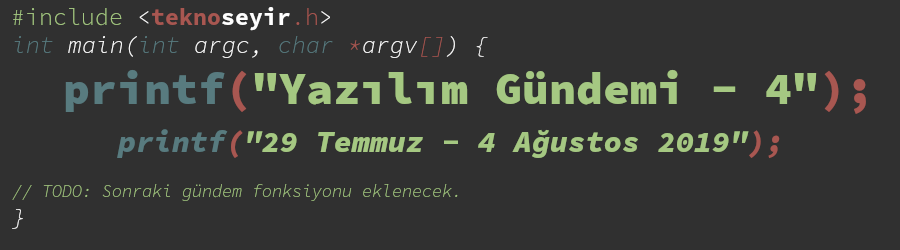
\includegraphics[width=.9\linewidth]{gorseller/yazilim-gundemi-banner.png}
\end{center}
\begin{center}
\href{../03/yazilim-gundemi-03.pdf}{< Önceki Gündem} | \textbf{29 Temmuz - 4 Ağustos 2019} | \href{../05/yazilim-gundemi-05.pdf}{Sonraki Gündem >}

\href{https://teknoseyir.com/blog/yazilim-gundemi-4-29-temmuz-4-agustos-2019}{TeknoSeyir'de Oku}
\end{center}

\section{Go dili topluluğu, dile generic programlama özellikleri eklemeyi \href{https://github.com/golang/go/issues/15292}{tartışıyor}}
\label{sec:org21c0b8a}
C\# yazdığım zamanlardan hatırladığım kadarıyla generic programlama terimi,
tipi belli olmayan fonksiyon parametreleri tanımlamak için kullanılıyordu.
Örnek vererek daha iyi anlatırım:

C++'da generic programlama ile şu şekilde bir yapı kurabiliyoruz.

\begin{minted}[breaklines=true,breakanywhere=true,frame=lines, linenos, label=C++, labelposition=topline]{cpp}
template <typename T>
class Liste {
  // sınıf içeriği
};

class Hayvan { };
class Araba { };

int main() {
  auto hayvan_listesi = new Liste<Hayvan>();
  auto araba_listesi = new Liste<Araba>();
}
\end{minted}

Bu yapının avantajı hem bizi kod tekrarından kurtarıyor, hem de işimizi
kolaylaştırıyor. Bu yapı sayesinde, atıyorum bu listelerin içeriklerini
yazdırmak istersek, parametre olarak \texttt{T} alan bir fonksiyon kodladığımızda, o
fonksiyona bu listelerin ikisini de gönderebiliyoruz.

Go dili topluluğu da, bu özelliği Go diline Contracts ile eklemeyi konuşuyor.
\href{https://go.googlesource.com/proposal/+/master/design/go2draft-contracts.md}{İlgili tavsiye sayfası}nda detaylıca anlatılmış.
\section{Ruby on Rails \href{https://weblog.rubyonrails.org/2019/7/30/Rails-6-0-rc2-released/}{6.0.0 RC2 yayınlandı}}
\label{sec:orga84f1ee}
Bu yılın başlarında \href{https://weblog.rubyonrails.org/2019/1/18/Rails-6-0-Action-Mailbox-Action-Text-Multiple-DBs-Parallel-Testing/}{6.0.0 beta1 sürümü duyurulan} popüler Ruby framework
sistemi Ruby on Rails, bu hafta içerisinde \href{https://weblog.rubyonrails.org/2019/7/30/Rails-6-0-rc2-released/}{6.0.0 rc2 sürümünü duyurdu}.

6.0.0 sürümü ile gelecek özelliklerden bazıları şunlar:
\begin{itemize}
\item Action Mailbox
\item Action Text
\item Çoklu veritabanı desteği
\item Paralel test çalıştırma desteği
\end{itemize}

Diğer özellikler için \href{https://weblog.rubyonrails.org/2019/1/18/Rails-6-0-Action-Mailbox-Action-Text-Multiple-DBs-Parallel-Testing/}{bu sayfayı} ziyaret edebilirsiniz.
\section{Windows Terminal \href{https://devblogs.microsoft.com/commandline/windows-terminal-preview-v0-3-release/?WT.mc\_id=social-reddit-marouill}{ön izleme sürümü v0.3 duyuruldu}}
\label{sec:org4c96ec9}
Uzun bir süredir geliştiriciler tarafından pek tercih edilmeyen Windows, artık
bazı şeyleri değiştirerek geliştiricileri kendine çekmeyi planlıyor gibi.
Bunlardan biri de o eski hantal, kullanışsız ve özelleştirme desteği çok az
olan terminal uygulaması. Bir süredir Microsoft'un bu uygulama üzerinde
çalıştığını biliyoruz. Zaten duyurdukları ilk ön izleme sürümü de bu değil.
Bu ön izleme sürümü ile gelen bazı yeni özellikler şu şekilde:

\subsection{Taşınabilir başlık çubuğu}
\label{sec:orgdd3ad4e}
Bu özelliği anlamadım önceden pencere taşınamıyor muydu yani, yeni mi geldi?
İlginç.

\url{gorseller/draggable.gif}
\subsection{Sekmeler kısmındaki açılır menünün yeri değişmiş}
\label{sec:org3b62f23}
Eski sürümde böyleyken:
\begin{center}

\includegraphics[width=.9\linewidth]{gorseller/title-bar-v02-1.png}
\end{center}

Artık bu hale gelmiş:
\begin{center}

\includegraphics[width=.9\linewidth]{gorseller/title-bar-v03.png}
\end{center}

Diğer özellikler için konu başlığındaki bağlantıya tıklayabilirsiniz. Açıkcası
bir terminal sever olarak Windows'a yeni modern bir terminal arayüzü gelmesine
sevindim fakat bu saatten sonra GNU/Linux tarafından tekrar Windows'a geri
dönmem çok zor. Yine de Windows üzerinde çalışan arkadaşlar adına sevindim.
\section{Firefox 68 ile gelen \href{https://hacks.mozilla.org/2019/07/new-css-features-in-firefox-68/}{yeni CSS özellikleri}}
\label{sec:orgee8e256}
Firefox tarayıcısının bu ay başında duyurulan 68 numaralı sürümü ile bazı yeni
CSS özellikleri de kullanıma açılmış. Bunlardan birisi şu şekilde:

\subsection{\texttt{::marker} ile listelerin maddelerini özelleştirme}
\label{sec:org583a9db}
Bildiğimiz gibi HTML'de iki çeşit liste tipi var. Birisi \texttt{ul}, yani Unordered
List (Sırasız Liste); diğeri ise \texttt{ol}, yani Ordered List (Sıralı Liste).
Artık bu çeşit listenin de madde işaretlerini CSS ile özelleştirebileceğiz.
Şöyle ki:

\begin{minted}[breaklines=true,breakanywhere=true,frame=lines, linenos, label=CSS, labelposition=topline]{css}
ul ::marker {
    color: hotpink;
}
ol ::marker {
    color: blue;
    font-size: 200%;
}
\end{minted}

Sonuç işe şu şekilde oluyor:
\begin{center}
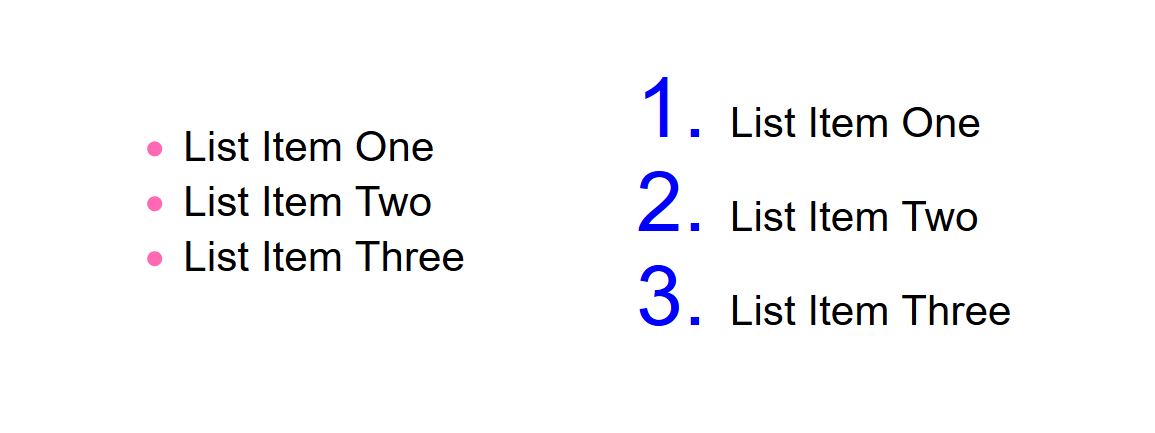
\includegraphics[width=.9\linewidth]{gorseller/css-market.png}
\end{center}

Diğer CSS özellikleri için \href{https://hacks.mozilla.org/2019/07/new-css-features-in-firefox-68/}{bu sayfayı} ziyaret edebilirsiniz.
\section{Bootstrap 3 desteği \href{https://blog.getbootstrap.com/2019/07/24/lts-plan/}{sonlandırıldı}}
\label{sec:org9011227}
Aslında bu geçen haftanın haberi fakat gözden kaçmış ama yine de değinmeden
geçmek istemedim. Tasarım cahili bir back-end developer olarak çok işime
yaramış, kendisiyle nice siteler hazırlamıştım fakat artık Bootstrap 3 sürümü
emekliye ayrılıyor. Artık güvenlik güncelleştirmeleri de gelmeyecek.

Bootstrap ekibi yeni uzun dönem desteklerini (LTS) Bootstrap 4 sürümü ile
devam ettireceklerini duyurdu.

Elveda Bootstrap 3\ldots{}
\section{Diğer Haberler}
\label{sec:org87be24d}
\begin{itemize}
\item Yazılım ile ilgili yeni bir Türkçe podcast serisi başladı: \href{https://www.youtube.com/watch?v=Pi4YaFXgYRE}{Pantalks}.
\item Çankırı Sağlık İl Müdürlüğü Bilgi Sistemleri, Windows Aktif Dizin Yapısıyla
entegre çalışan \href{https://github.com/Cankirism/ADManager}{AD Yönetim uygulaması}nın ilk sürümünü \href{https://twitter.com/csmbilsis/status/1157205580672622592}{açık kaynak olarak
yayınladı}.
\item Laravel Türkiye forumları \href{https://laravel.gen.tr/d/3383-laravel-turkiye-forumlari-yenilendi}{yenilendi}.
\item Android Studio \href{https://androidstudio.googleblog.com/2019/08/android-studio-35-release-candidate-2.html}{3.5 RC2 sürümü duyuruldu}.
\item \href{https://gitea.io/}{Gitea} \href{https://blog.gitea.io/2019/07/gitea-1.9.0-is-released/}{1.9.0 sürümünü yayınladı}.
\item JavaScript ile platformlar-arası (cross-platform) masaüstü uygulamalar
geliştirmeye yarayan \href{https://electronjs.org/}{Electron} kütüphanesinin \href{https://electronjs.org/blog/electron-6-0}{6.0.0 sürümü duyuruldu}.
\item \href{https://crystal-lang.org/}{Crystal} programlama dilinin \href{https://crystal-lang.org/2019/08/01/crystal-0.30.0-released.html}{0.30.0 sürümü duyuruldu}.
\item Amazon, tüm veritabanı sistemleri için tek bir sorgu dili olma iddiasını
taşıyan \href{https://aws.amazon.com/tr/blogs/opensource/announcing-partiql-one-query-language-for-all-your-data/}{yeni aracını duyurdu}: \href{https://partiql.org/}{PartiQL}, \href{https://github.com/partiql/partiql-lang-kotlin}{GitHub Deposu}.
\item MSDN Magazine \href{https://msdn.microsoft.com/en-us/magazine/mt833502.aspx?f=255\&MSPPError=-2147217396}{yayın hayatına son verdi}.
\item Microsoft, proje örneklerinin listenebileceği \href{https://docs.microsoft.com/en-us/teamblog/code-samples}{yeni bir sayfa yayınladı}:
\url{https://docs.microsoft.com/samples}.
\item ASP.NET takımı, RESTful HTTP hizmetleri ile etkileşime geçmeyi sağlayan yeni
komut satırı aracını duyurdu: \href{https://devblogs.microsoft.com/aspnet/httprepl-a-command-line-tool-for-interacting-with-restful-http-services/}{HttpRepl}, \href{https://github.com/aspnet/HttpRepl}{GitHub Deposu}.
\item EmacsConf sanal konferansı için \href{https://emacsconf.org/2019/cfp}{konuşmacı çağrısı yayınladı}.
\item GNU C (glibc) kütüphanesinin \href{https://lwn.net/Articles/795127/}{2.30 sürümü yayınlandı}.
\item OpenJDK takımı, \href{https://openjdk.java.net/projects/loom/}{Loom projesi}nin \href{https://mail.openjdk.java.net/pipermail/loom-dev/2019-July/000633.html}{erken erişim sürümlerini duyurdu}.
\item Sunucuyu test etmek için yük oluşturmak amacıyla kullanılan \href{https://github.com/Gymmasssorla/anevicon}{anevicon} isimli
aracın \href{https://github.com/Gymmasssorla/anevicon/releases/tag/v7.0.0}{v7.0.0 sürümü duyurdu}.
\item Ruby kütüphanesi ROM (Ruby Object Mapper), \href{https://rom-rb.org/blog/rom-5-1-released/}{5.1 sürümü yayınlandı}.
\item Go ile yazılmış paralel görüntü işleme algoritmalarının toplandığı \href{https://github.com/anthonynsimon/bild}{bild}
isimli proje \href{https://github.com/anthonynsimon/bild/releases/tag/0.11.0}{v0.11.0 sürümünü yayınladı}.
\item Go ile yazılmış, shell komutları için görselleştirme imkanı sunan \href{https://github.com/sqshq/sampler}{Sampler}
isimli proje, \href{https://github.com/sqshq/sampler/releases/tag/v1.0.0}{ilk stabil sürümünü duyurdu}.
\item Git depolarınızı takip eden ve duruma göre \texttt{pull} veya \texttt{push} yapan araç
açık kaynak olarak yayınlandı: \href{https://github.com/muesli/gitomatic}{git-o-matic}.
\item Tamamen merkezsizleştirilmiş (decentralized) anahtar-değer (key-value) depo
aracı LF, \href{https://github.com/zerotier/lf/releases/tag/0.9.20.0}{0.9.20.0 sürümünü duyurdu}.
\item Makine öğrenmesi modellerini JSON API olarak kullanmaya olanak sağlayan araç
\href{https://cortex.dev/}{Cortex}, \href{https://github.com/cortexlabs/cortex/releases/tag/v0.7.0}{v0.7.0 sürümü yayınlandı}.
\item Yapay sinir ağları temelli elastic search aracı \href{https://github.com/gnes-ai/gnes}{GNES}, \href{https://github.com/gnes-ai/gnes/releases/tag/v0.0.26}{v0.0.26 sürümünü
yayınladı}.
\item Java ile PDF oluşturma ve düzenleme kütüphanesi \href{https://github.com/LibrePDF/OpenPDF}{OpenPDF} \href{https://github.com/LibrePDF/OpenPDF/releases/tag/1.3.0}{1.3.0 sürümünü
duyurdu}.
\item \href{https://github.com/cettia/asity}{Asity} \href{https://cettia.io/blog/asity-3-0-0-released/}{3.0.0 sürümü duyuruldu}.
\item \href{https://github.com/blobcity/db/}{BlobCityDB} veritabanının \href{https://github.com/blobcity/db/releases}{1.7.9 sürümü duyuruldu}.
\item Sadece 512 byte ile BASIC dilini çalıştırabilen interpreter projesi
\href{https://github.com/nanochess/bootBASIC}{bootBASIC} yayınlandı.
\item Yeni bir etiketleme dili ortaya çıktı: \href{https://github.com/jeml-lang/jeml}{JEML}
\end{itemize}
\section{Lisans}
\label{sec:orgdfece51}
\begin{center}
\begin{center}

\includegraphics[height=1.5cm]{../../../img/CC_BY-NC-SA_4.0.png}
\end{center}

\href{yazilim-gundemi-04.pdf}{Yazılım Gündemi - 4} yazısı \href{https://erenhatirnaz.github.io}{Eren Hatırnaz} tarafından \href{http://creativecommons.org/licenses/by-nc-sa/4.0/}{Creative Commons
Atıf-GayriTicari-AynıLisanslaPaylaş 4.0 Uluslararası Lisansı} (CC BY-NC-SA 4.0)
ile lisanslanmıştır.
\end{center}
\end{document}
